\documentclass{../../../oss-apphys-exam}
\usepackage{enumitem}
\newcounter{last}

\begin{document}

\gentitle{1}{ELECTROSTATICS, PART 1}

\raggedcolumns

\runningheader{
  \fontfamily{phv}\small
  \textcolor{gray}{AP PHYSICS C: ELECTRICITY AND MAGNETISM $\blacksquare$}
  \textbf{MULTIPLE-CHOICE QUESTIONS}}{}{}


\begin{multicols*}{2}
  \begin{questions}
    \question Two fixed charges $A$ and $B$ are separated by a distance $r$.
    The electric force on charge $B$ by charge $A$ has a magnitude $F$. Which
    of the following statement(s) \textbf{must} be correct?
    \begin{enumerate}[label=\Roman*.]
    \item The electric force on charge $A$ by charge $B$ has a magnitude $F$.
    \item The magnitude of charge of $A$ and $B$ are the same.
    \item When distance $r$ is doubled, $F$ is halved.
    \end{enumerate}
    \begin{choices}
      \choice I only
      \choice II only
      \choice I and III only
      \choice I, II and III
      \choice None of the the above statements are correct
    \end{choices}
    \uplevel{
      \centering
      \vspace{.1in}
      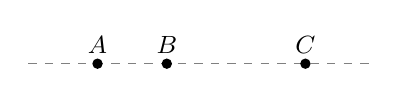
\begin{tikzpicture}[scale=1.1]
        \draw[dashed,gray] (0,0)--(4,0);
        \fill (.8,0) circle (.06) node[above]{\small$A$};
        \fill (1.6,0) circle (.06) node[above]{\small$B$};
        \fill (3.2,0) circle (.06) node[above]{\small$C$};
      \end{tikzpicture}
    }
    \question Three point charges, $A$, $B$ and $C$ are fixed along a straight
    line, as shown in above figure. The resultant electric force on charge $B$
    is zero. Which of the following statement(s) \textbf{must} be correct?
    \begin{enumerate}[label=\Roman*.]
    \item Charge $A$ carries a charge of the same sign as charge $C$.
    \item The electric force on charge $B$ by charge $A$ is half of that by
      charge $C$.
    \item The magnitude of charge carried by charge $C$ is 4 times that of
      charge $A$.
    \end{enumerate}
     \begin{choices}
      \choice I only
      \choice II only
      \choice I and III only
      \choice II and III only
      \choice None of the the above statements are correct
    \end{choices}
    
    \question A positive charge is placed on a spherical conducting hollow shell
    of radius $R$. Which of the following statements is true?
    \begin{choices}
      \choice The charge is distributed evenly on the inside surface of the
      sphere.
      \choice The charge is distributed evenly on the outside surface of the
      sphere.
      \choice The charge is concentrated at the center of the sphere.
      \choice The inside surface of the sphere is negatively charged.
      \choice The charge is concentrated at the poles on the surface of the
      sphere.
    \end{choices}
  
    \question A positive charge is placed on a solid conducting sphere of radius
    $R$. Which of the following statements is true?
    \begin{choices}
      \choice The electric field is zero everywhere inside the sphere.
      \choice The electric field is zero just outside the surface of the sphere.
      \choice The electric field is maximum at the center of the sphere.
      \choice The electric field is directed radially outward outside the
      surface of the sphere.
      \choice The electric field inside the sphere is equal and opposite to
      the electric field outside the surface of the sphere.
    \end{choices}
  
    \uplevel{
      \textbf{Questions \ref{cond1}--\ref{cond2}}: A positive charge $Q$ is
      placed at the center of a hollow conducting sphere.
      \begin{center}
        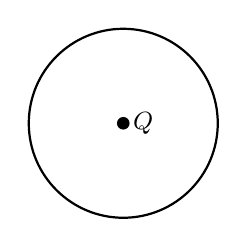
\begin{tikzpicture}
          \draw[thick] circle (1.2);
          \fill circle (.08) node[right]{\small$Q$};
        \end{tikzpicture}
      \end{center}
    }
  
    \question The charge on the inside surface of the hollow sphere is
    \begin{choices}
      \choice $-Q$
      \choice $+Q$
      \choice $-2Q$
      \choice $+2Q$
      \choice zero
    \end{choices}
    \label{cond1}
  
    \question A grounding wire is connected to the sphere, and then removed. The
    charge on the sphere is now
    \begin{choices}
      \choice $-Q$
      \choice $+Q$
      \choice $-2Q$
      \choice $+2Q$
      \choice zero
    \end{choices}
    \label{cond2}
    \columnbreak

    \uplevel{
      \textbf{Questions \ref{pair1}--\ref{pair2}}: An electron and a proton are
      released from rest in free space. The attract each other due to the
      electrical force on them
    }
    \question Which of them will have a larger magnitude of momentum when they
    collide?
    \label{pair1}
    \begin{choices}
      \choice The proton
      \choice The electron
      \choice Both will have the same magnitude of momentum
      \choice There is not enough information to determine
    \end{choices}

    \question Which of them will have more kinetic energy when they collide?
    \label{pair2}
    \begin{choices}
      \choice The proton
      \choice The electron
      \choice Both will have the same amount of kinetic energy
      \choice There is not enough information to determine
    \end{choices}
    
    \uplevel{
      \centering
      \begin{tikzpicture}
        \foreach \x in {0,1,2} \draw[axes] (\x,1)--(\x,-1);
        \draw[ultra thick] (.5,0)--(1.5,0);
        \shade[ball color=gray!50] (.5,0) circle(.15) node[above]{\small$+4Q$};
        \shade[ball color=gray!50] (1.5,0) circle(.09) node[above]{\small$-Q$};
      \end{tikzpicture}
    }
    \question Two charges, $+4Q$ and $-Q$, are connected by an insulated rod and
    rest in a uniform electric field $\vec E$ as shown. Ignore the effects of
    gravity on the charges and rod. The rod and charges will experience
    \begin{choices}
      \choice a clockwise rotation and a downward acceleration
      \choice a counterclockwise rotation and a downward acceleration
      \choice a clockwise rotation and an upward acceleration
      \choice a counterclockwise rotation and an upward acceleration
      \choice no rotation, but a downward acceleration
    \end{choices}
  
    \question An electron and a proton are separated by \SI{1.50e-10}\metre. If
    they are released, which one will accelerate at a greater rate, and what is
    the magnitude of that acceleration?
    \begin{choices}
      \choice The electron; \SI{1.12e22}{m/s^2}
      \choice The proton; \SI{1.12e22}{m/s^2}
      \choice The electron; \SI{6.13e18}{m/s^2}
      \choice The proton; \SI{6.13e18}{m/s^2}
      \choice They both accelerate at the same rate; \SI{1.02e-8}{m/s^2}
    \end{choices}
    \columnbreak
    
    \question Eight identical charges $q$ are fixed on the vertices of a cube
    of side length $\ell$. The resultant force on each one of the charges is
    $F$. If the cube now expands, and the new side length becomes $2\ell$, what
    is the resultant force on each positive charge?
    \begin{choices}
      \choice $F$
      \choice $2F$
      \choice $4F$
      \choice $F/2$
      \choice $F/4$
    \end{choices}
    
    \question Four charges are arranged at the corners of a square of side a as
    shown. Which of the following is true of the electric field and the electric
    potential at the center of the square?
    \begin{center}
      \begin{tikzpicture}[scale=1.75]
        \draw[dashed] (0,0)--(1,0)--(1,1) node[midway,right]{$a$}
        --(0,1)--cycle;
        \fill (.5,.5) circle (.03);
        \draw[fill=white] (0,0) circle (.05) node[below left]{$-q$};
        \draw[fill=white] (1,0) circle (.05) node[below right]{$+q$};
        \draw[fill=white] (0,1) circle (.05) node[above left]{$+q$};
        \draw[fill=white] (1,1) circle (.05) node[above right]{$-q$};
      \end{tikzpicture}
    \end{center}
    \begin{tabular}{rcc}
      & \underline{Electric Field} & \underline{Electric Potential}\\
      (A) & zero & zero \\
      (B) & $\dfrac{kQ}{a\sqrt 2}$ & zero \\
      (C) & $\dfrac{kQ^2}{2a^2}$ &  $\dfrac{kQ}{2a}$\\
      (D) & zero &  $\dfrac{kQ}{\sqrt{2a}}$\\
      (E) & $\dfrac{kQ^2}{2a}$ & $\dfrac{kQ}{a\sqrt 2}$
    \end{tabular}
    \columnbreak
    
    \question Which of the following diagrams best represents how you might
    rearrange the charges so that the electric field at the center would point
    directly toward the top of the page?
    
    \begin{oneparchoices}
      \choice
      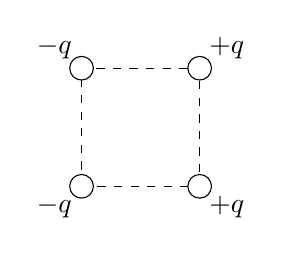
\begin{tikzpicture}[scale=1.5]
        \draw[dashed] rectangle (1,1);
        \draw[fill=white] circle (.1) node[below left]{$-q$};
        \draw[fill=white] (1,0) circle (.1) node[below right]{$+q$};
        \draw[fill=white] (0,1) circle (.1) node[above left]{$-q$};
        \draw[fill=white] (1,1) circle (.1) node[above right]{$+q$};
      \end{tikzpicture}
      \choice
      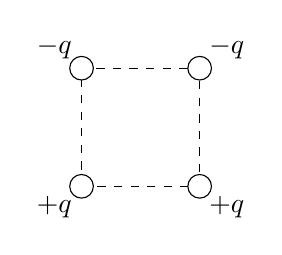
\begin{tikzpicture}[scale=1.5]
        \draw[dashed] rectangle (1,1);
        \draw[fill=white] circle (.1) node[below left]{$+q$};
        \draw[fill=white] (1,0) circle(.1) node[below right]{$+q$};
        \draw[fill=white] (0,1) circle(.1) node[above left]{$-q$};
        \draw[fill=white] (1,1) circle(.1) node[above right]{$-q$};
      \end{tikzpicture}
      \choice
      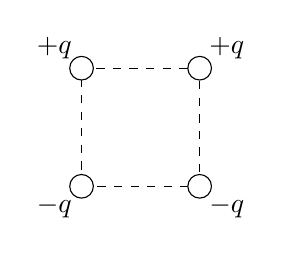
\begin{tikzpicture}[scale=1.5]
        \draw[dashed] rectangle (1,1);
        \draw[fill=white] circle (.1) node[below left]{$-q$};
        \draw[fill=white] (1,0) circle (.1) node[below right]{$-q$};
        \draw[fill=white] (0,1) circle (.1) node[above left]{$+q$};
        \draw[fill=white] (1,1) circle (.1) node[above right]{$+q$};
      \end{tikzpicture}
      \choice
      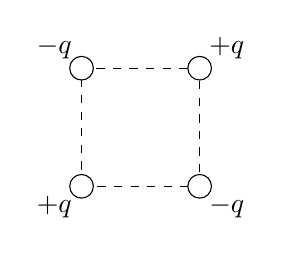
\begin{tikzpicture}[scale=1.5]
        \draw[dashed] rectangle (1,1);
        \draw[fill=white] circle (.1) node[below left]{$+q$};
        \draw[fill=white] (1,0) circle (.1) node[below right]{$-q$};
        \draw[fill=white] (0,1) circle (.1) node[above left]{$-q$};
        \draw[fill=white] (1,1) circle (.1) node[above right]{$+q$};
      \end{tikzpicture}
      \choice
      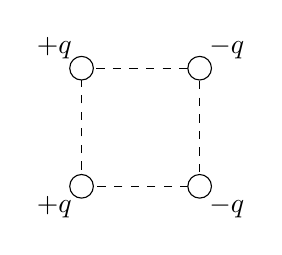
\begin{tikzpicture}[scale=1.5]
        \draw[dashed] rectangle (1,1);
        \draw[fill=white] circle (.1) node[below left]{$+q$};
        \draw[fill=white] (1,0) circle (.1) node[below right]{$-q$};
        \draw[fill=white] (0,1) circle (.1) node[above left]{$+q$};
        \draw[fill=white] (1,1) circle (.1) node[above right]{$-q$};
      \end{tikzpicture}
    \end{oneparchoices}
    \columnbreak
    
    \question Three charges, $+Q$, $-Q$, and $+2Q$, are arranged in an
    equilateral triangle as shown. Which of the arrows below best represents the
    direction of the electric field at the center of the triangle?
    \begin{center}
      \vspace{-.1in}
      \begin{tikzpicture}[scale=2]
        \draw[dashed](0,0)--(1,0)--(.5,.866)--cycle;
        \draw (.5,.289) circle (.03);
        \draw[fill=white] circle (.05) node[left] {$+Q\;$};
        \draw[fill=white] (1,0) circle (.05) node[right]{$\;-Q$};
        \draw[fill=white] (.5,.866) circle (.05) node[above]{$2Q$};
      \end{tikzpicture}
    \end{center}
    \begin{choices}
      \choice {\Huge$\downarrow$}
      \choice {\Huge$\uparrow$}
      \choice {\Huge$\searrow$}
      \choice {\Huge$\swarrow$}
      \choice {\Huge$\nearrow$}
    \end{choices}
  \end{questions}
  \setcounter{last}{\value{question}}
\end{multicols*}
\newpage

%\genfreetitle{14}{ELECTROSTATICS}{3}
%\genfreedirections


  % USED FOR FALL-WINTER-SPRING TERM IN 2021, BUT THIS HAS BEEN MOVED TO
  % PHYSICS 12 AND AP PHYSICS 2 HOMEWORK INSTEAD
  
%  \question In the Bohr model of the hydrogen atom, the electron moves in a
%  circular orbit of radius $r$ around the proton.
%  \begin{parts}
%    \part Find an expression for the kinetic energy of the electron as a
%    function of $r$. Show that at any distance $r$, the kinetic energy and
%    potential energy have a ratio of $-1/2$.
%    \part Evaluate kinetic energy $K$, potential energy $U$ and the total
%    energy $E=K+U$ in electron volts for\\ $r=\SI{0.529e-10}\metre$, the
%    radius of the electron's orbit in hydrogen. (The energy $|E|$ that must be
%    supplied to the hydrogen atom to remove the electron is called the
%    ionization energy.)
%  \end{parts}
%  \newpage

\runningheader{
  \fontfamily{phv}\small
  \textcolor{gray}{AP PHYSICS C: MECHANICS $\blacksquare$}
  \textbf{FREE-RESPONSE QUESTIONS}}{}{}


% TAKEN FROM 2023 AP PHYSICS C E&M EXAM SET 1 FREE-RESPONSE QUESTION 1
% MODIFIED FROM THE STANDARD QUESTION
\begin{center}
  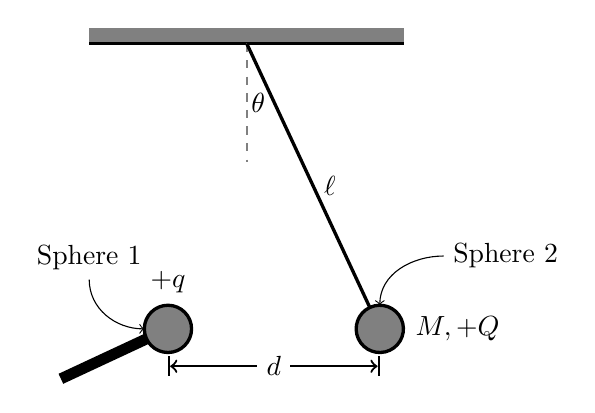
\begin{tikzpicture}
    \fill[gray](-2,0) rectangle (2,.2);
    \draw[very thick] (-2,0)--(2,0);
    \draw[thick,dashed,gray] (0,0)--(0,-1.5)
    node[midway,right=-2,black]{$\theta$};
    \begin{scope}[rotate=25,very thick]
      \draw (0,0)--(0,-4) node[midway,right]{$\ell$};
      \draw[fill=gray] (0,-4) circle (.3) node[right=9]{$M,+Q$};
    \end{scope}
    \fill[rotate around={25:(-1,-4*cos{25})}]
    (-1,-4*cos{25}-.07) rectangle (-2.5,-4*cos{25}+.07);
    \draw[very thick,fill=gray] (-1,-4*cos{25}) circle (.3) node[above=9]{$+q$};
    \draw[|<->|,thick] (-1,-4.1)--(4*sin{25},-4.1) node[midway,fill=white]{$d$};

    \draw[<-] (-1.3,-4*cos{25}) to[out=180,in=270] (-2,-3)
    node[above]{Sphere 1};

    \draw[<-] (4*sin{25},.3-4*cos{25}) to[out=90,in=180] (2.5,-2.7)
    node[right]{Sphere 2};
  \end{tikzpicture}
\end{center}

\begin{questions}
  \setcounter{question}{\value{last}}
  
  \question Students perform an experiment to determine the value of vacuum
  permittivity $\varepsilon_0$. Sphere 1 is nonconducting with charge $+q$ and
  is attached to an insulating rod. Sphere 2 is nonconducting with charge $+Q$
  and has mass $M$. Sphere 2 is hung from a string of negligible mass and
  length $\ell$. Sphere 1 is brought near, without touching, Sphere 2, as shown
  above. Equilibrium is established when the centers of the two spheres have
  the same vertical position, are a horizontal distance $d$ apart, and the
  string is at an angle $\theta$ from the vertical.

  \begin{parts}
    \part On the following dot that represents Sphere 2 at the position shown
    in the previous figure, \textbf{draw} and \textbf{label} the forces (not
    components) that act on Sphere 2. Each force must be represented by a
    distinct arrow starting on, and pointing away from, the dot.
    \uplevel{
      \centering
      \begin{tikzpicture}
        \draw[thick,dashed] (-2,0)--(2,0);
        \draw[thick,dashed] (0,-2)--(0,2);
        \fill circle (.3);
      \end{tikzpicture}
    }

    \part\textbf{Derive} the relationship between the distance $d$ and the angle
    $\theta$ to show that
    $d = \sqrt{\dfrac{Qq}{4\pi\varepsilon_0Mg\tan\theta}}$
    \vspace{\stretch1}
    
    \part These values are collected in one trial: $Q=q=\SI{6.0e-8}\coulomb$,
    $\theta=\SI{12}\degree$, and $d=\SI{.057}\metre$. \textbf{Calculate} the
    expected force of tension exerted on Sphere 2 by the string.
    \vspace{\stretch1}
    \newpage

    \uplevel{
      The students vary $d$ and measure $\theta$ after equilibrium is reached.
      The students use the collected data to plot the following graph of
      $d^2$ vs.\ $\dfrac1{\tan\theta}$.
      \begin{center}
        \begin{tikzpicture}[scale=1.7]
          \draw[axes] (0,0)--(6.5,0) node[right]{$\dfrac1{\tan\theta}$};
          \draw[axes] (0,0)--(0,5.5) node[above]{$d^2$ [\si{\metre^2}]};
          \draw[step=.25,gray,dashed] (0,0) grid (6,5);
          \draw (0,0) grid (6,5);

          \foreach \x in {0,2,...,12} \draw(\x/2,0)--+(0,-.1) node[below]{$\x$};
          \foreach \y in {0.000,0.002,...,0.010}
          \draw(0,\y*500)--+(-.1,0) node[left]{$\y$};

          \fill (1.82,1.25) circle (.04);
          \fill (2.82,1.78) circle (.04);
          \fill (3.55,2.45) circle (.04);
          \fill (4.25,3.2) circle (.04);
          \fill (5.72,4.04) circle (.04);
        \end{tikzpicture}
      \end{center}
      
    }


    \part \textbf{Draw} the best-fit line for the data.
    \part Using the best-fit line, \textbf{calculate} an experimental value for
    the vacuum permittivity $\varepsilon_0$ when $M=\SI{.0050}{\kilo\gram}$ and
    $Q=q=\SI{6.0e-8}\coulomb$.
    \vspace{\stretch1}
    \newpage
    
    \uplevel{
      The students modify the experiment by replacing Sphere 1 with a
      conducting Sphere 3 that has the same size and charge $+q$. The
      experiment is repeated.
    }
    
    \part The circle in the following figure represents Sphere 3 when spheres
    2 and 3 are at equilibrium. On the circle, \textbf{draw} a single ``$+$''
    sign to represent the location of highest concentration of the excess
    positive charges.
    \label{conductor}
    \uplevel{
      \centering
      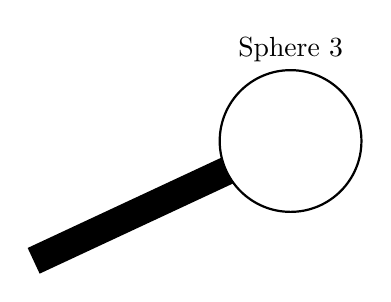
\begin{tikzpicture}[scale=.9]
        %\draw[thick,dashed] (-2,0)--(2,0);
        \fill[rotate=25] (0,.2) rectangle (-4,-.2);
        \draw[thick,fill=white] circle (1) node[above=25]{Sphere 3};
      \end{tikzpicture}
    }
    \part Briefly \textbf{explain} your reasoning for the sketch drawn in part
    \textbf{F}.
    \vspace{\stretch1}
    
    \part In the original experiment, when the centers of the two spheres are a
    horizontal distance $d_1$ apart, the string makes an angle $\theta_1$ from
    the vertical. In the modified experiment, when the centers of the two
    spheres are a horizontal distance $d_1$ apart, the string makes an angle
    $\theta_2$ from the vertical. Is $\theta_2$ greater than, less than, or
    equal to $\theta_1$?

    \vspace{.15in}
    \underline{\hspace{.3in}} $\theta_2 > \theta_1$ \hspace{.3in}
    \underline{\hspace{.3in}} $\theta_2 < \theta_1$ \hspace{.3in}
    \underline{\hspace{.3in}} $\theta_2 = \theta_1$ 

    \vspace{.15in}\textbf{Justify} your answer.
    \vspace{\stretch1}
  \end{parts}
  \newpage
    
  % TAKEN FROM 2021 AP PHYSICS C E&M EXAM FREE-RESPONSE QUESTION 1
  \uplevel{
    \centering
    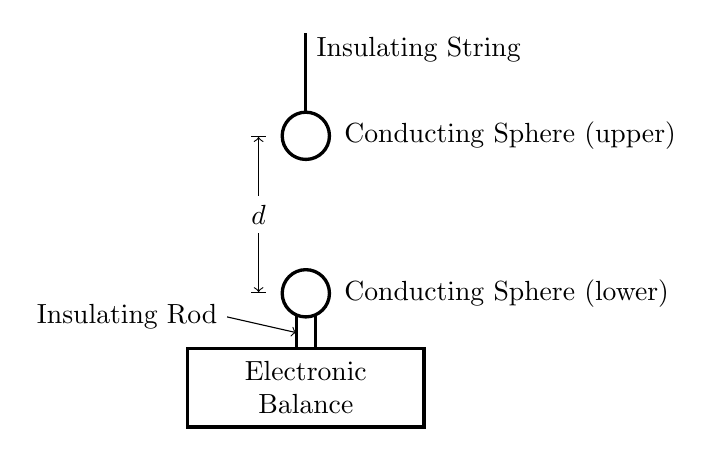
\begin{tikzpicture}
      \begin{scope}[very thick]
        \draw circle (.3) node[right=10]{Conducting Sphere (upper)};
        \draw (0,.3)--+(0,1) node[pos=.8,right]{Insulating String};

        \draw (-.12,-2.2) rectangle +(.24,-.5);
        \draw[fill=white] (0,-2) circle(.3)
        node[right=10]{Conducting Sphere (lower)};

        \draw (-1.5,-2.7) rectangle +(3,-1)
        node[midway,text width=50,align=center]{Electronic\\Balance};
      \end{scope}
      \draw[<-] (-.12,-2.5)--(-1,-2.3) node[left]{Insulating Rod};
      \draw[|<->|] (-.6,0)--+(0,-2) node[midway,fill=white]{$d$};
    \end{tikzpicture}
  }

  \question Students perform an experiment to study the force between two
  charged objects using the apparatus shown above, which contains two identical
  conducting spheres. The upper sphere is attached to an insulating string,
  which can be used to move the sphere downward. The lower sphere sits on an
  insulating rod, which is on an electronic balance. The electronic balance is
  zeroed \emph{before} the lower sphere and insulating rod are in place.

  \vspace{.15in}For the first trial, a charge of $Q$ is placed on each sphere
  and then the upper sphere is slowly moved downward. The students measure the
  distance $d$ between the centers of the spheres and the magnitude $F$ of the
  force that appears on the electronic balance. The recorded data are shown on
  the graph of $F$ as a function of $\dfrac1{d^2}$ shown below. 
  \uplevel{
    \centering
    \begin{tikzpicture}[scale=1.7]
      \draw[axes] (0,0)--(5.5,0)
      node[right]{$\dfrac1{d^2}$ [\si{\per\metre\squared}]};
      \draw[axes] (0,0)--(0,4.2) node[above]{$F$ [\si{\milli\newton}]};
      \draw[dashed,step=.25] grid (5,4);
      \draw[thick] grid (5,4);
      \foreach \x in {0,20,...,100} \draw (\x/20,0)--+(0,-.1) node[below]{$\x$};
      \foreach \y in {9,10,...,13}
      \draw (0,\y-9)--+(-.1,0) node[left]{$\y$};
    \end{tikzpicture}
  }
  \begin{parts}
    \part\textbf{Draw} a line that represents the best fit to the points
    shown.

    \part Use the graph to \textbf{calculate} the charge $Q$.
    \vspace{\stretch1}
    \newpage
    
    \part On the graph, \textbf{draw} a circle around the data point that was
    taken when the distance between the centers of the spheres was the least.
      
    \part Determine the distance between the centers of the spheres for the
    data point indicated above.
    \vspace{\stretch1}

    \part What physical quantity does the vertical intercept represent?
    \textbf{Justify} your answer.
    \vspace{\stretch4}
    \newpage
      
    \uplevel{
      \cpic{.7}{real-data}
      
      The experiment is extended by collecting additional data points, which
      appear on the right side of the graph shown above. The new data points
      do not follow the linear pattern seen with the first points. The group
      of students tries to explain this discrepancy.
    }
    \part One student suspects that charge is slowly leaking off the top
    sphere. Could this explain the discrepancy?

    \vspace{.15in}
    \underline{\hspace{.25in}} Yes\hspace{.5in}
    \underline{\hspace{.25in}} No
          
    \vspace{.15in}\textbf{Justify} your answer.
    \vspace{\stretch1}

    \part A second student suspects that the excess charges have rearranged
    themselves, polarizing the spheres.
    \begin{subparts}
      \subpart On the circles representing the spheres below, \textbf{draw} a
      single ``$+$'' sign on each sphere to represent the locations of highest
      concentration of the excess positive charges.
      \uplevel{
        \centering
        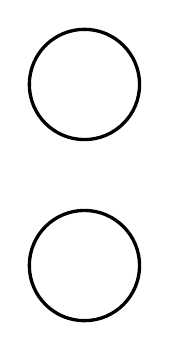
\begin{tikzpicture}[very thick]
          \draw circle (.7);
          \draw (0,-2.3) circle (.7);
        \end{tikzpicture}
      }
      \subpart\textbf{Explain} how this rearrangement could be responsible for
      the discrepancy.
      \vspace{\stretch1}
    \end{subparts}
    \newpage
      
    \part A third student suggests that the experiment be modified so that
    the top sphere is given a negative charge that is equal in magnitude to
    the positive charge given to the bottom sphere.

    \begin{subparts}
      \subpart On the circles representing the spheres below, \textbf{draw} a
      single ``$+$'' sign on the bottom sphere to represent the location of
      highest concentration of the excess positive charges. Use a single
      ``$-$'' sign on the top sphere to represent the location of the highest
      concentration of the excess negative charges.
      \uplevel{
        \centering
        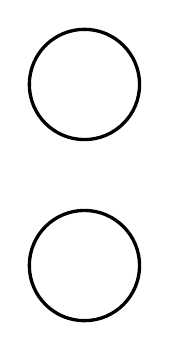
\begin{tikzpicture}[very thick]
          \draw circle (.7);
          \draw (0,-2.3) circle (.7);
        \end{tikzpicture}
      }
      \subpart For a separation distance equal to that of the data point
      indicated in part \textbf{B}, would the magnitude of the force reading
      with spheres of opposite charges be greater than, less than, or equal
      to the magnitude of the force reading with spheres of the same charges?

      \vspace{.15in}
      \underline{\hspace{.25in}} Greater than\hspace{.35in}
      \underline{\hspace{.25in}} Less than\hspace{.35in}
      \underline{\hspace{.25in}} Equal to

      \vspace{.15in}\textbf{Justify} your answer.
      \vspace{\stretch1}
    \end{subparts}
  \end{parts}
%  \newpage
%  
%  \question A spherically symmetric charge distribution has net positive charge
%  $Q_0$ distributed within a radius of $R$. Its electric potential $V$ as a
%  function of the distance $r$ from the center of the sphere is given by the
%  following
%  \begin{align*}
%    V(r) &= \frac{Q_0}{4\pi\epsilon_0R}\left[-2+3\left(\frac rR\right)^2 \right]
%    \text{ for } r<R\\
%    V(r) &= \frac{Q_0}{4\pi\epsilon_0r}\text{ for } r>R
%  \end{align*}
%  Express all algebraic answers in terms of the given quantities and
%  fundamental constants.
%  \begin{parts}
%    \part For the following regions, indicate the direction of the electric
%    field $E(r)$ and derive an expression for its magnitude.
%    \begin{subparts}
%      \subpart $r < R$
%      
%      \vspace{.1in}\underline{\hspace{.4in}} Radially inward
%        
%      \vspace{.1in}\underline{\hspace{.4in}} Radially outward
%      \vspace{\stretch1}
%      
%      \subpart $r > R$
%      
%      \vspace{.1in}\underline{\hspace{.4in}} Radially inward
%
%      \vspace{.1in}\underline{\hspace{.4in}} Radially outward
%      \vspace{\stretch1}
%      
%    \end{subparts}
%    
%    \part For the following regions, derive an expression for the enclosed
%    charge that generates the electric field in that region, expressed as a
%    function of $r$.
%    \begin{subparts}
%      \subpart $r < R$
%      \subpart $r > R$
%    \end{subparts}
%    \vspace{\stretch1}
%    \newpage
%    \part Is there any charge on the surface of the sphere ($r=R$)?
%
%    \vspace{.1in}
%    \underline{\hspace{.4in}} Yes\hspace{.3in}
%    \underline{\hspace{.4in}} No
%    
%    If there is, determine the charge. In either case, explain your reasoning.
%    \vspace{\stretch1}
%    
%    \part On the axes below, sketch a graph of the force that would act on a
%    positive test charge in the regions $r<R$ and $r > R$. Assume that a force
%    directed radially outward is positive.
%    \begin{center}
%      \begin{tikzpicture}[scale=1.1]
%        \draw[very thick,->](0,-3)--(0,3) node[above]{$F$};
%        \draw[very thick,->](0,0)--(10,0) node[right]{$r$};
%        \draw[dashed](4,-3)--(4,3) node[midway,below left]{$R$};
%      \end{tikzpicture}
%    \end{center}
%  \end{parts}
%  \vspace{\stretch1}
\end{questions}
\end{document}
